\chapter{Introduction}\label{Chap1}
\echapter{Introduction}

\section{Background}\label{Chap1_01}
\esection{Background}
In the microelectronics industry, the chip technology is rapidly evolving towards miniaturization in accordance to the Moore's law. Owing to this miniaturization trend in the chip technology, the reliability of solder joints used in the electronic packaging has been considered as a significant topic.  

\section{Motivation}\label{Chap1_01}
\esection{Motivation}

Today, most of the recently launched mobile devices are equipped with a set of embedded sensors and multiple wireless interfaces such as Bluetooth, Wi-Fi, and cellular radio. These devices are now capable of supporting ad-hoc communication mode and researchers begin to consider social features to design networking solutions. As a result, the field of socially aware networking~\cite{FXia2013} is emerged as a new paradigm. This paradigm can be applied into many areas such as ad-hoc social networks, pocket switched networks~\cite{SWang2012}, vehicular ad hoc networks~\cite{WChen2008}, cyber-physical systems (CPS)~\cite{FJWu2011}, etc.

Ad-hoc Social Networks (ASNETs) are the combination of social networks and Mobile Ad-hoc Networks (MANETs) as shown in Fig. 1.1. This networking area is different from Mobile Social Networks (MSNs)~\cite{NKayastha2012}. MSNs are the combination of social networks and simply mobile networks. ASNETs have a dynamic topology because of users' mobility while MSNs do not have such dynamic nature. In other words, the dynamicity or node mobility in MSNs is limited or it's not the primary goal of the network. Based on the network structure, ASNETs have an opportunistic (ad-hoc or delay tolerant) nature whereas mobile social networks are both centralized and opportunistic, even if sometimes with blurred borders.
\begin{figure}[b]
\begin{center}
  \begin{tabular}{c}
  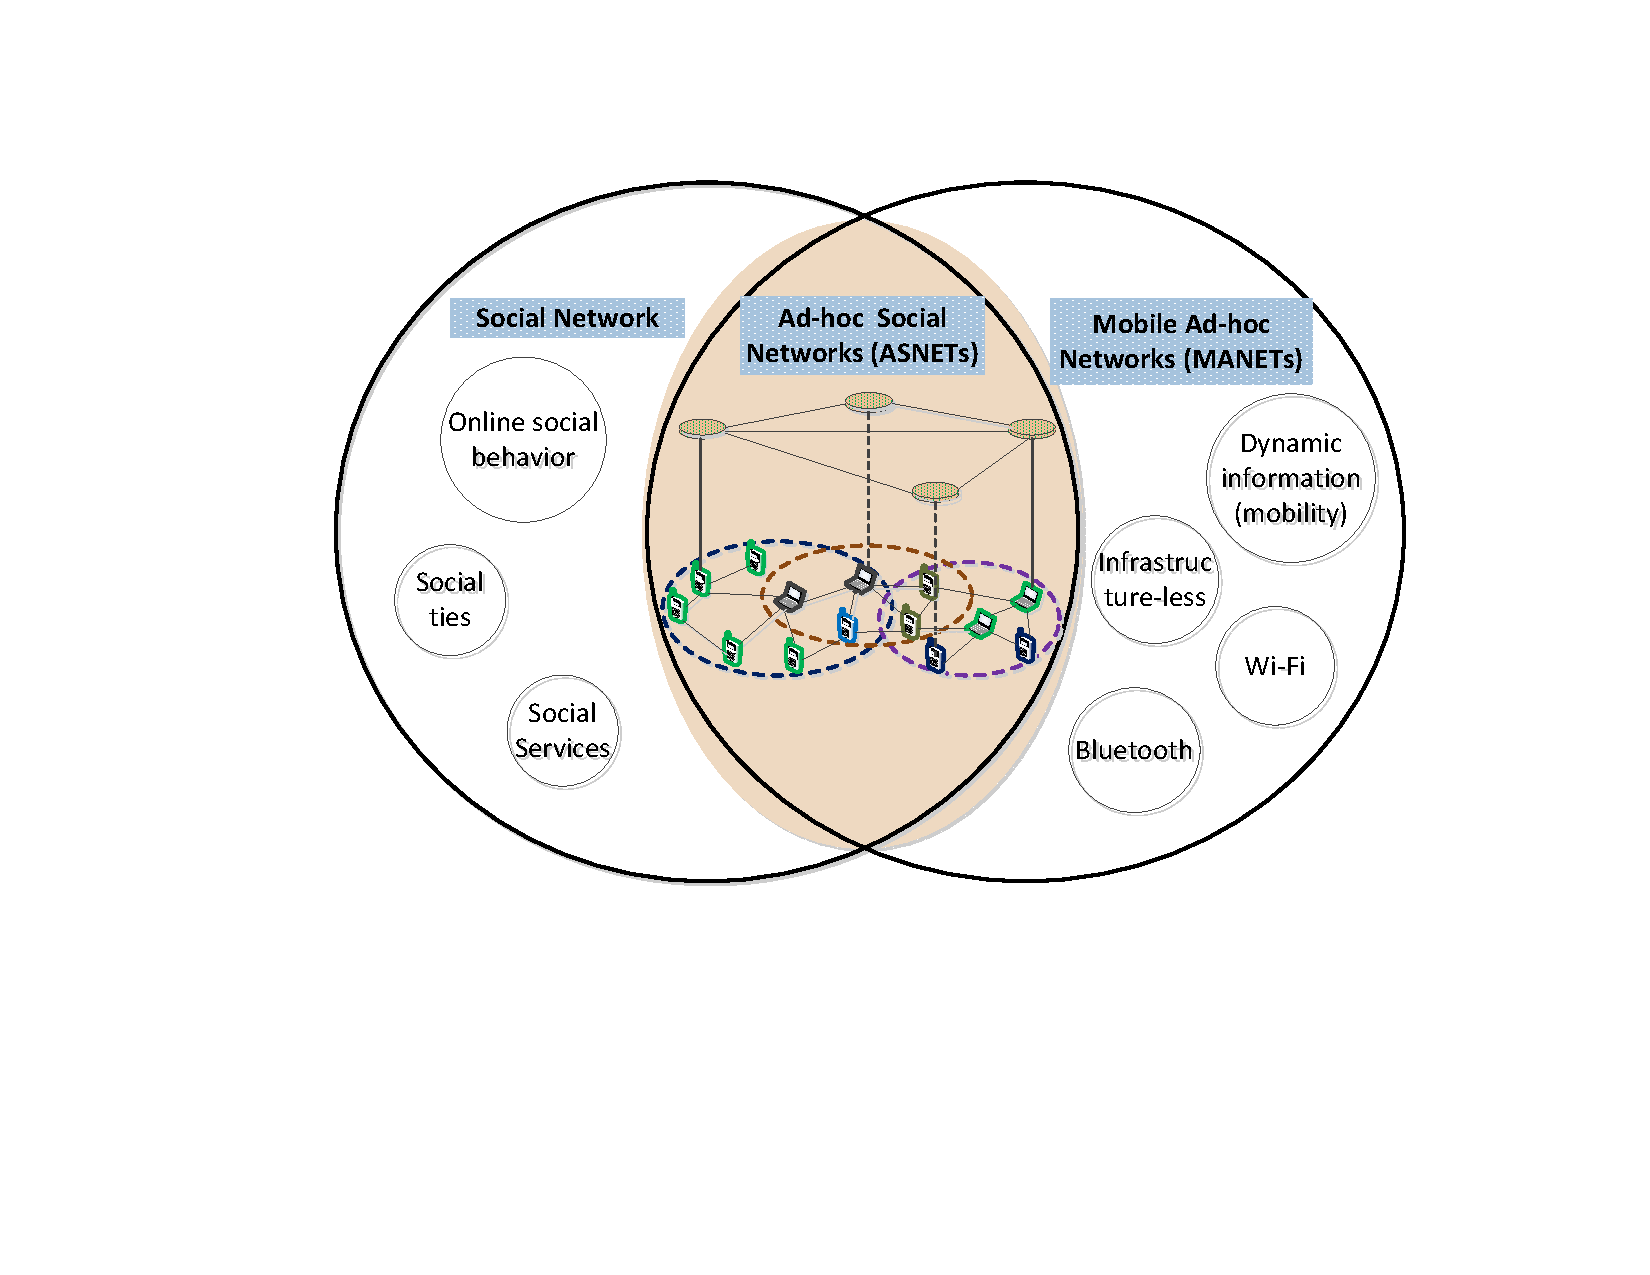
\includegraphics[width=0.65\textwidth]{Chap1-Fig1.pdf}
  \end{tabular}
  \caption{Ad-hoc social networks at the intersection of social networks and mobile ad-hoc networks.}
\end{center}
\end{figure}

This presents a new research area related to data publishing, dissemination, exchange, sharing, and delivery services by learning and analyzing the data collected using different sensing technologies~\cite{RKGanti2011}. In a broader sense, ASNET is a mobile ad-hoc communications system which involves the social behavior of the users. In such a network, mobile users can access, share, and distribute data in a mobile environment by exploiting the social interactions. Due to the ubiquitous availability of sensor enabled mobile devices (such as smart phones); an ASNET can fully take advantage of human interaction and physical mobility to achieve efficient and effective data delivery services.

Although the potential of using emerging ad-hoc networking technologies for middleware design and development has been discussed for a number of years now in both industrial and research communities, until recently there has been little or no advancement in the field of ad-hoc social networks. All that is changing because of a number of important technological advances such as the introduction of social behaviors~\cite{FXia2013}, rise of socially-aware opportunistic sensing~\cite{HJohnson2011} and mobile phone sensing~\cite{NDLane2010}, emergence of Social Community Intelligence (SCI)~\cite{DZhang2012} and mobile cloud~\cite{NFernando2013}. The combination of these advances to ad-hoc networking solutions opens the gate for new innovative approaches and will lead to the development of middleware for ASNETs.

In fact, this new research field can leverage results and insights from sensing, intelligent devices (such as machine learning and data mining), social behaviors; it still presents new technical challenges for middleware design which are not addressed yet. Socially-aware networks involve a great deal of information, such as personal property (e.g., preference, habit, and life regularity), human-to-human relationship (e.g., friendship, colleague, and family), human-to-community relationship (e.g., interests and popularity), and human-to-environment relationship. By exploiting these social behaviors which are collected from the sensing technologies, its objective is to design service solutions to support mobile applications such as smart conference. In such a system, data dissemination \& replication strategies and routing \& forwarding protocols are the most important components by which data are distributed. In addition, they involve essential components such as resource management and reliability. While relatively a few efforts have been made in the past few years on related issues for MSNs and MANETs, the whole area of middleware design for socially-aware networks particularly ASNETs is still at an early phase compared with other relatively mature areas in wireless networks.

There are many interesting research problems in ad-hoc networks. Some of these are unique as the middleware developed for traditional mobile wireless networks can't be directly applied to ASNETs due to the salient characteristics such as user online behavior, user mobility and limited resource generally and some are similar to research problems that are currently being addressed by researchers and developers. One of the problems that are unique to mobile ad-hoc networking is performance degradation and implementation inefficiencies that are caused by the gap between application layer and lower layer protocols. Also, some existing middleware schemes in this networking environment are designed for specific scenario and are not adaptive enough to be used in different network environments. Moreover, some of these rely directly or indirectly on static nodes or fixed wireless network infrastructure for their operation. Due to these specific properties that come into play on the network, it makes an interesting research topic to study the design of a layer (middleware) supporting coordination between the upper and lower layer protocols. A distributed middleware for different ASNET scenarios are now feasible due to the use of data management, which is the most important task. Such data management middleware allows a network to operate more efficiently and predictably under a broader range of varying conditions.

Replication is an important mechanism in modern wireless networks and has attracted significant efforts to improve its performance with different metrics including read cost, network traffic, consistency, relocation cost, etc. Traditionally, different ideal approaches are widely used to facilitate data availability. However, the quality of wireless links would be affected by many factors like mobility and overhead. The availability, accessibility and reliability of ASNET services can be assured by replica allocation and management approaches. Therefore, the first of the three proposed protocols addresses data replication to increase data availability by putting copy of data items locally or nearby. In such a situation, replication helps to avoid data losses in case of an unpredictable group mobility that causes community partition and also aids in reducing the number of hops when a data is transmitted from source to destination. We propose a new replica allocation method that can significantly improve the network performance taking social relationships and properties of its data into account while replicating in the community to achieve better efficiency and consistency by keeping the replica relocation cost as low as possible. This type of replica allocation method will increase the availability and accessibility of different data items in a partitioned social community.

The proposed replica allocation method for ASNETs does have merits in dealing with the problem of storage overload. However, a major shortcoming is the assumption that load for a storage space is proportional to the amount of data (original or replica), stored in the same space. In other words, the load balance computation module doesn't consider the inter-community loads and it can only be applied for very specific replication method. Due to this, it is important to design a load balancing approach in the broader sense of data dissemination. Load balancing is a well-established technique for utilizing available computing resources more effectively by partitioning tasks according to load distribution strategies. An uneven load distribution of real-world applications and the susceptibility of link failure in networks cause challenges of performance degradation and poor scalability. In our second protocol, partitioning and replication techniques have been implemented by exploring community-based load balancing to cope with such issues. Furthermore, the novel approach herein exploits offloading at the inter-community level as well as filter replication at the intra-community level. This results in the dynamic distribution and forwarding of publication and subscription services among brokers during run time.

Data management protocols for socially-aware networks assume that users are cooperative when participating in operations such as forwarding. In reality, however, some users are selfish.  Involvement of these selfish users can pose a serious threat to network performance and fairness, particularly in ASNETs. Therefore, it is essential to detect such selfish users and mitigate their impact on the performance of other well-behaving users. Finally, our third protocol adopts a bacterial bio-inspired technique to augment the replication protocol proposed initially with a mechanism to detect and counteract selfishness, to reduce the effect of selfish users in the network and provide better operations in an efficient way.

\section{Summary of Contributions}\label{Chap1_02}
\esection{Summary of Contributions}

The contributions of this dissertation, which are elaborated throughout this dissertation, are listed as follows:
\begin{enumerate}
    \item \textbf{ASNETs middleware framework}
    \\
    Middleware framework for wireless networks have been a topic of research for several years. However, there is no formal data management system framework to date that consolidates all current research in this area. This is considered a potential weakness of the research field. For example, the design of proposed data management protocols remains difficult, mainly due to the lack of system framework upon which the design could be based. Such system framework will provide the background for design and evaluation of middleware protocols. It will also help to provide metrics for assessing the effectiveness of an ASNET middleware protocol as well as its performance.
        \begin{itemize}
            \item We provide theoretical model of online social behavior and dynamic network information to represent the relationship between users using a social graph.
            \item We present a method to understand the social metrics usage of the protocols.
            \item we propose an ASNETs framework which integrates layers from sensing level to application level.
        \end{itemize}
    \item \textbf{Community partition aware data replication scheme for ASNETs with the exploitation of social relationships}
    \\
    A new data replication protocol called ComPAS (community-partition aware replica allocation method) is proposed initially. This method can significantly improve ASNETs performance by exploiting social relationship while replicating in the community to achieve better efficiency and consistency while keeping the replica relocation cost as low as possible.
        \begin{itemize}
            \item We model the data management middleware system for ASNETs with underlying different modules.
            \item We outline social relationship considerations as a social behavior for the exploitation of group mobility model.
            \item We provide an overview and selection on existing replica allocation approaches, that ease the impact of ASNETs connectivity nature and improve data availability ratio.
            \item We derive the average read cost for the original data storage space in a community without replication and also calculate the optimum Read Cost Reduction (RCR).
            \item We devise a replica allocation algorithm based on the proposed model and derived formulas.
            \item We choose an optimum approach and provide a comparison based on metrics such as read cost, relocation period, number of mobility group and efficiency of consistency management.
        \end{itemize}
    \item \textbf{An optimal community-based event dissemination with load balancing mechanisms for ASNETs }
    \\
    A community-based load balancing protocol called Co-Lab is proposed, that seeks to improve the network performance by clustering brokers in a community taking interest similarity and filter replication into consideration. It attempts to effectively achieve a more consistent and uniform load distribution among brokers and to circumvent the occurrence of highly overloaded brokers.
        \begin{itemize}
            \item We introduce a community-based event dissemination and load balancing with a fault-tolerance mechanism considering community formation, event dissemination, broker clustering based on interest similarity, replication, and load distribution.
            \item We design a possible load balancing algorithm by exploiting interest similarity and integrating filter-based functionality within each multicast group that achieves fair load distribution among each broker as well as reducing the overall load distribution.
            \item We formulate and derive the community formation system of the network and calculating the number of brokers, publishers and subscribers that should be involved in each community.
            \item We present an event dissemination algorithm for Inter-Community and Intra-Community phases, while balancing the load among brokers.
            \item We design a broker clustering and filter replication mechanism in the community.
            \item We conduct evaluation to verify the performance of the proposed approach. For evaluation, we generated an appropriate social graph model which substantiates the advantages of the socially-aware design of our system.
\end{itemize}
    \item \textbf{Bacteria social behavior inspired algorithm to detect and mitigate the impact of selfish users in ASNETs}
    \\
    A biologically inspired algorithm to detect and mitigate the impact of selfish users on performance and efficiency of ASNETs. Its design considers social willingness (that depends on depth of social relationship among users) as a social behavior and bacteria chemical products as a counter to achieve optimal ASNETs performance. Counter is a parameter attached to individual user counting successful data operations performed in relation with others. Using social willingness and counter, BoDMaS assesses and classifies users, and counteracts their selfishness.
        \begin{itemize}
            \item We model how to map the bacteria mechanism into our solution and how our solution is motivated by behavior of bacteria in performing collaborative tasks.
            \item We consider social willingness and a biologically inspired mechanism (chemical products of bacteria) in ASNET data replication operations to detect and classify users as either cooperative or selfish.
            \item We present a BoDMaS system architecture, which is made up of behavior assessment, user classification, and user selection \& reaction components.
            \item We demonstrate that the functional interaction among BoDMaS components can effectively detect selfishness.
            \item We conduct simulations by applying important performance and efficiency metrics such as accessibility degree, detection rates, and network load balance to validate the BoDMaS effectiveness.
\end{itemize}
\end{enumerate}

\section{Organization of the Dissertation}\label{Chap1_03}
\esection{Organization of the Dissertation}
\begin{figure}[h]
\begin{center}
  \begin{tabular}{c}
  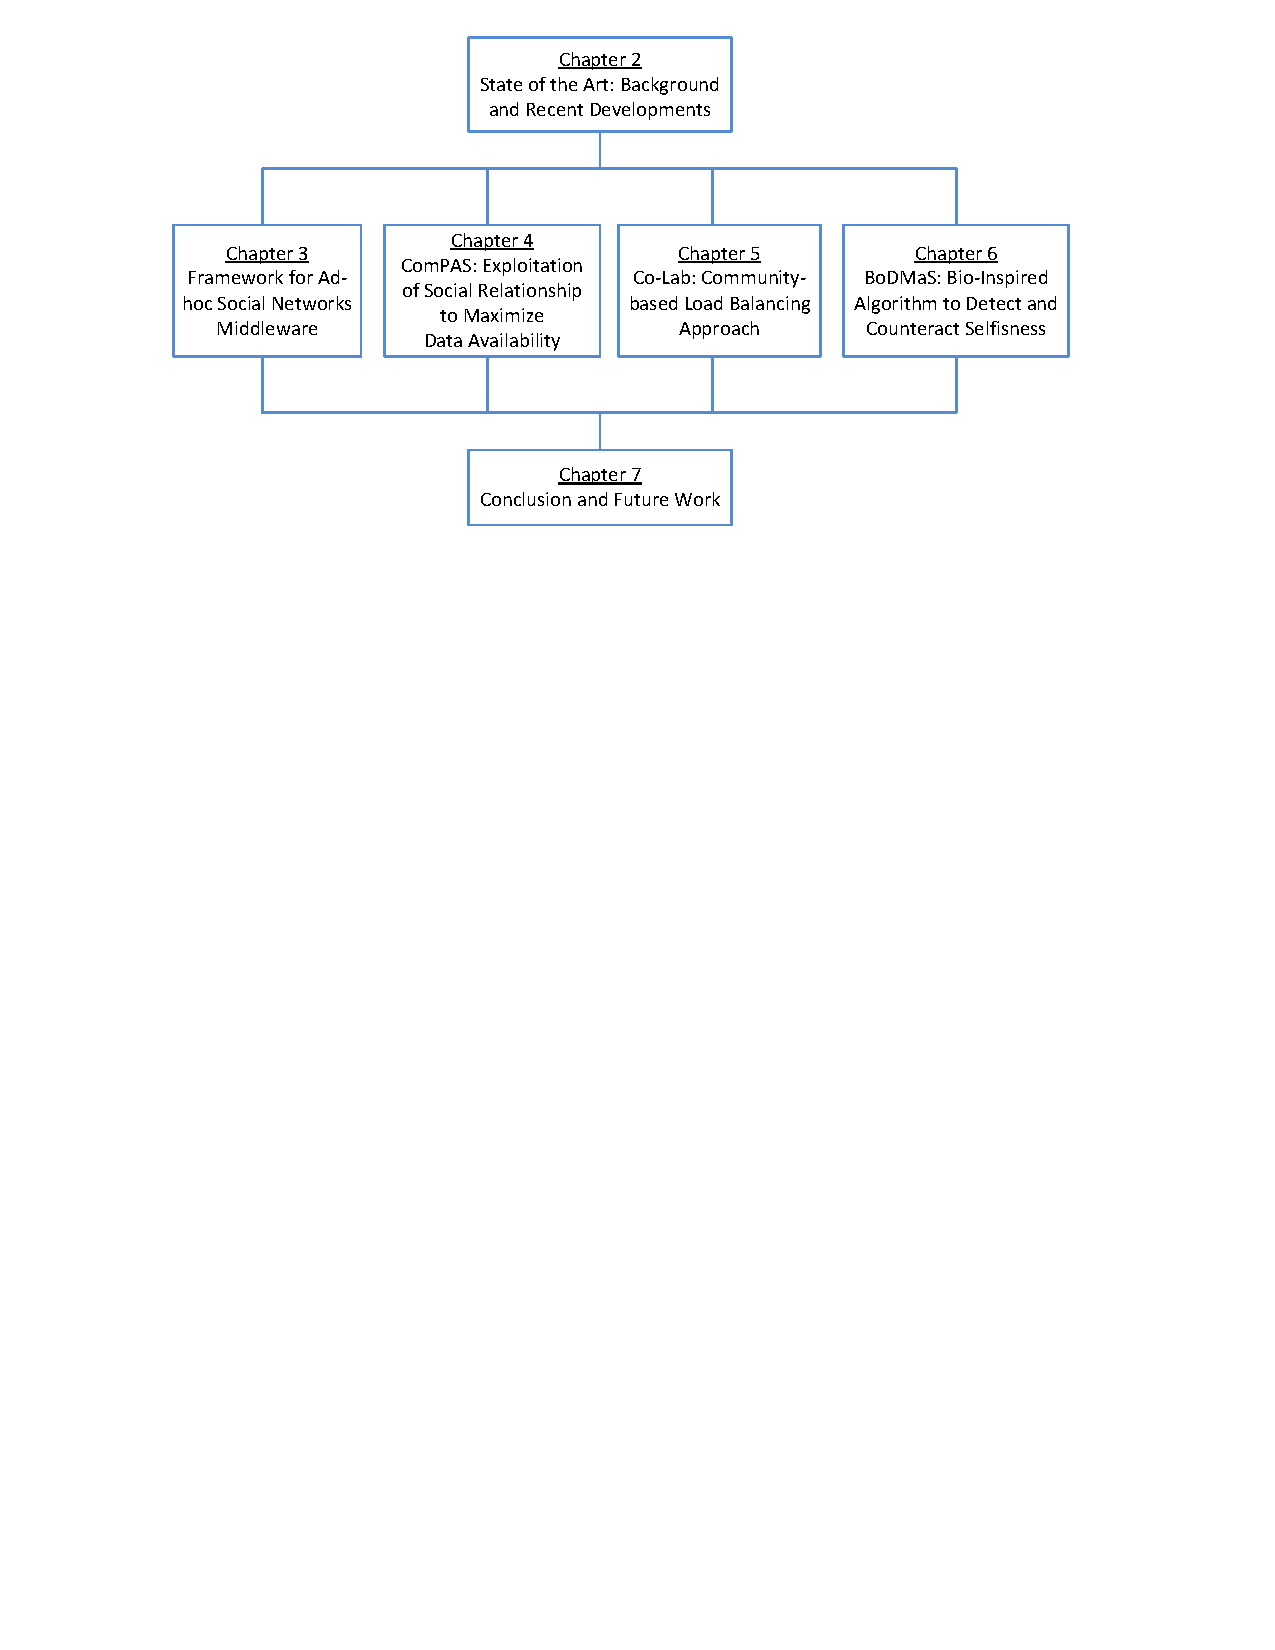
\includegraphics[width=0.856\textwidth]{Chap1-Fig2.pdf}
  \end{tabular}
  \caption{The organization of the remainder of the dissertation.}
\end{center}
\end{figure}
The remainder of the dissertation is organized as shown in Fig. 1.2: Chapter 2 lays a theoretical state of the art background for the following work, including introductions to user social behaviors, user mobility, middleware solutions for ad-hoc social networks, data replication, load balancing and user selfishness. Chapter 3 provides an ASNET middleware framework and overview of the relation of the layers as well as the protocols. Chapter 4 presents a social community partition aware replica allocation scheme that exploits users' relationship. In Chapter 5, we propose an optimal community-based load-balancing method. Chapter 6 provides bio-inspired algorithm to detect and counteract selfishness in ASNETs. Chapter 8 concludes the dissertation and discusses future research directions.

To provide an overall picture of the dissertation content, we created a dependency graph among chapters (Fig. 1.3) in which arrows suggest dependencies between chapters. Based on the dependency graph, therefore, a reader can start with Chapter 2 (state of the art: background and recent developments), and it is recommended that he or she read Chapters 3 (framework for ad-hoc social networks middleware) and 4 (ComPAS) before Chapter 5 (Co-Lab) and Chapter 6 (BoDMaS). We have also color-coded chapter boxes that are of the same level of importance and abstraction. The darkest chapters are the essentials of this dissertation, and the lightest boxes are those chapters that are more applied and have materials that are built on the foundation of other chapters.

\begin{figure}[h]
\begin{center}
  \begin{tabular}{c}
  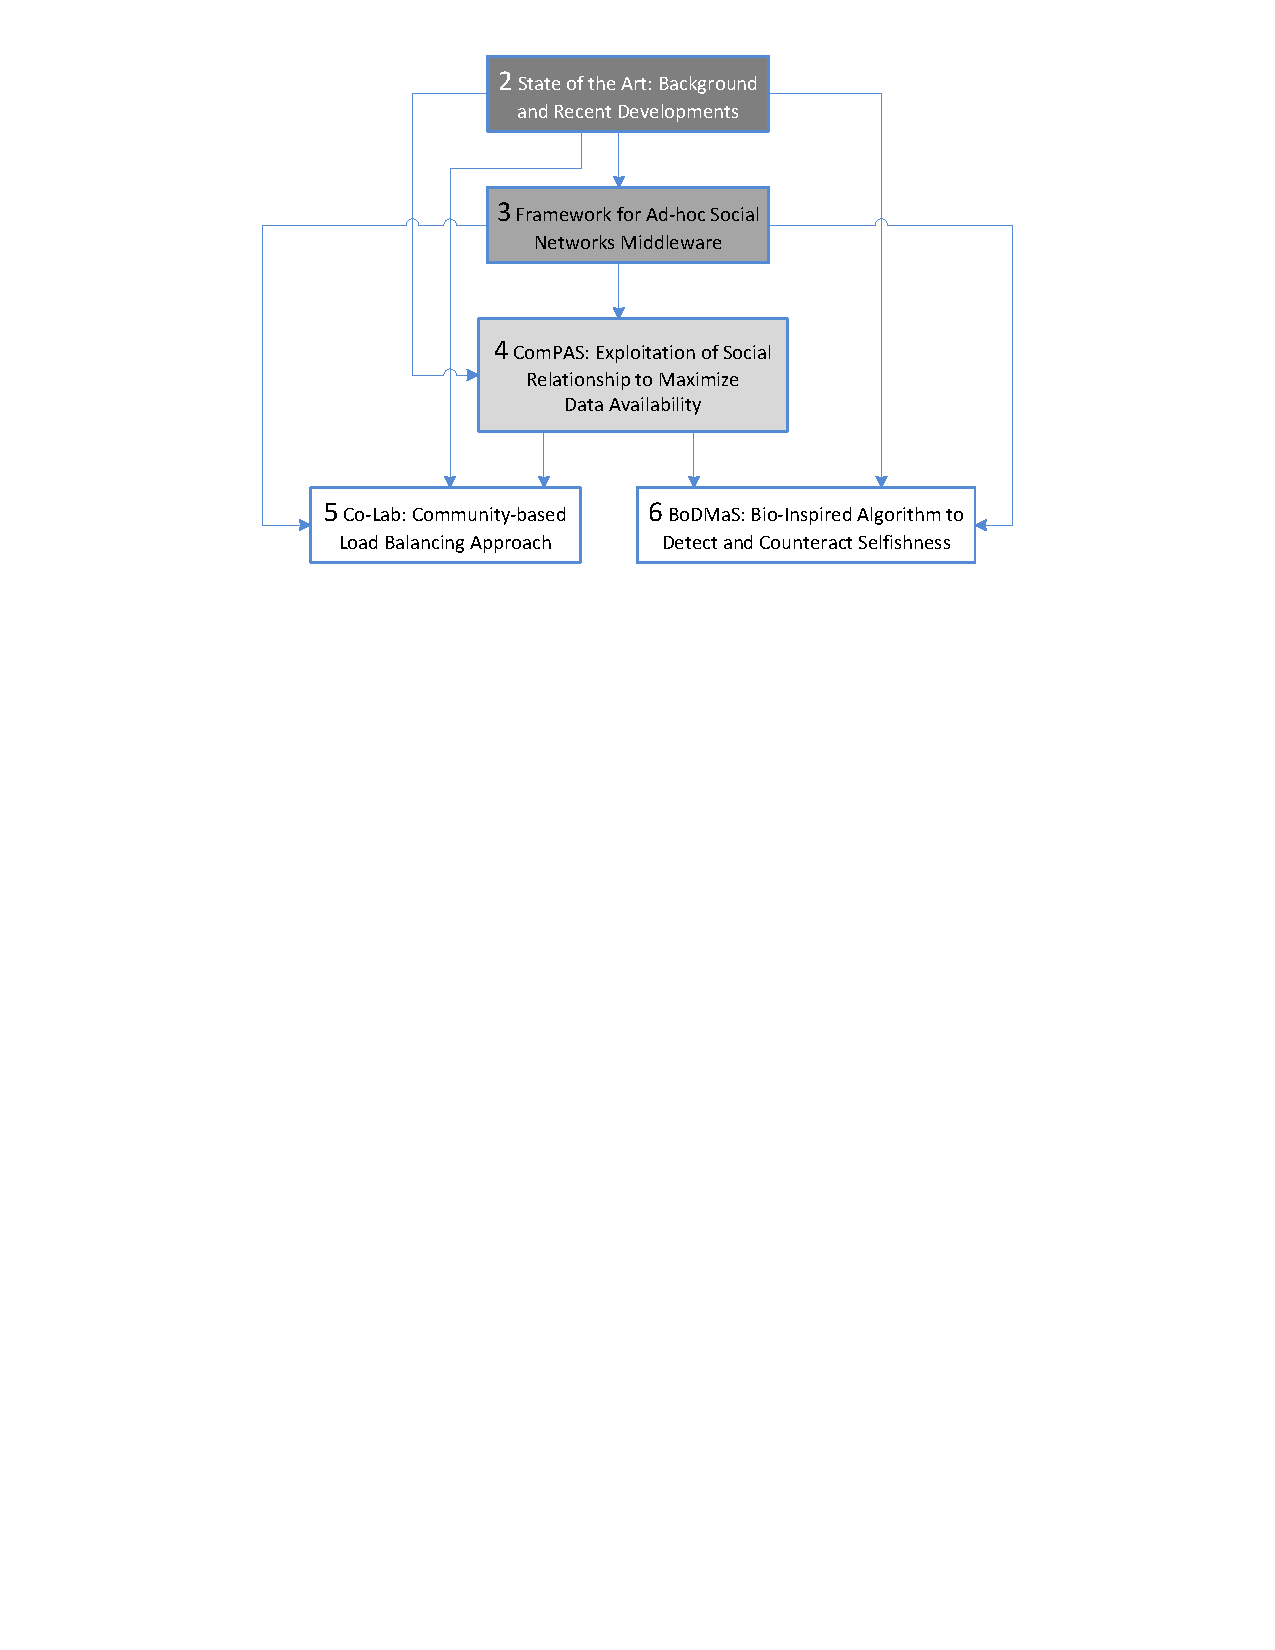
\includegraphics[width=0.75\textwidth]{Chap1-Fig3.pdf}
  \end{tabular}
  \caption{Dependency between dissertation Chapters. Arrows show dependencies and colors represent chapter levels.}
\end{center}
\end{figure}
